\chapter{Introduction}
\label{introchap}

\section{Motivation}
\sectionmark{Motivation}

\subsection{Convection in astrophysics: Stars \& Beyond}
\label{sct:convective_abundance}
In nature, thermal buoyancy forces primarily drive two types of flows: gravity waves and convection.
Gravity waves are driven when the atmospheric or fluid stratification is convectively \emph{stable}.
Convection is the opposite, and is the manifestation of these buoyancy forces in the presence of an \emph{unstable} or \emph{superadiabatic} stratification.
Convection occurs in the Earth's atmosphere, and cumulus clouds are evidence of that convection (and there is a rich literature investigating atmospheric convection, see \citet{yano2014} for a recent review).
The Earth's mantle convects \citep{schubert&all2001}, driving plate tectonics \citep{bercovici2003}, and the earth's outer core convects, driving the Earth's magnetic dynamo \citep{christensen2011}.
Convection also accurs in more exotic astrophysical systems, including in the planes of accretion disks \citep{held&latter2018} and in the magnetospheres of giant planets \citep{thomsen&all2012}.
The prevelance of convective motions across astrophysics suggests that an intricate understanding of the fundamental nature of convection is crucial.

One of the most classical and well-studied examples of astrophysical convection is convection in stars.
The surface of the Sun is covered in convective ``granules,'' and these granules are evidence of a convection zone that occupies the outer 30\% of the Sun's radial profile \citep{miesch2005, nordlund&all2009}.
The Sun is not the only Main Sequence (MS) star to rely on convection to transport a part of its luminosity.
``Early-type'' or ``Upper-MS'' high-mass stars ($M \gtrsim 1.5 M_\odot$, where $M_\odot$ is the solar mass) have convecting regions in their cores.
In these massive stars, core conditions are sufficiently extreme that the CNO cycle is activated.
The opacity of the stellar material, dominated by free-free interactions \citep[c.f.~Ch.~16 of][]{weiss&all2004}, is sufficiently high that the extreme CNO-fed luminosities cannot be efficiently carried by radiative processes.
Convection is therefore required to transport the stellar luminosity outward, and results in a well-mixed convective core region.
The luminosity of stars with masses smaller than $1.5 M_\odot$ is provided by the pp-chain, and these stars have stable cores.
However, these stars also have cooler surface temperatures which allow for phase changes of hydrogen and helium within their stellar envelopes.
These elements are the primary consitutents of the stellar material, and unionized atoms greatly increase the stellar opacity through bound-free (photo effect) interactions \citep[these effects were first studied in detail by ][]{rast&toomre1993a, rast&toomre1993b}.
In solar-type stars ($1.5 M_\odot \lesssim M \lesssim 0.3 M_\odot$), this increased opacity near the stellar surface results in a convectively unstable envelope which overlies a stable, radiative interior.
In ``Late-type'', ``Lower-MS'' stars, these opacity effects lead to convective instability throughout the full depth of the star.
While stars spend the majority of their lifetimes on the MS, convection is also an important process during other evolutionary phases \citep[and I refer the reader to chapter 2 of][for a broad but brief overview of stellar evolutionary phases]{HKT}.

The relatively new fields of helioseismology and asteroseismology (briefly explored in Sct.~\ref{sct:asteroseismology}) have enabled scientists to literally look inside of the Sun and stars.
These measurements allow us to put constraints upon and test the validity of stellar structure models, and our assumptions about the workings of stellar interiors.
In Sct.~\ref{sct:convective_conundrum}, I briefly discuss the ``Solar Convective Conundrum,'' one of the discrepancies between models and observations that has been revealed by helioseismology.
In short, this conundrum shows that our fundamental understanding of stellar convection is flawed.
The collection of experiments presented in this thesis were largely motivated by this Conundrum, and a desire to rebuild some understanding of stellar convection from fundamental principles.

\subsection{Asteroseismology \& Helioseismology}
\label{sct:asteroseismology}
Stars are seismically active.
This seismic activity is the manifestation of complex, 3D oscillations within the star which come in two primary forms: pressure-driven ``p''-modes, and buoyancy-driven ``g''-modes.
The simplest of these modes are radial modes, in which the star experiences spherically symmetric oscillations along its radial coordinate (and the simplest of these modes is the fundamental ``breathing'' mode, in which the star's radius expands and contracts as a whole).
On top of these radial modes, nonradial modes (including dipolar, quadrupolar, and infinitely more complex modes) are also excited.
As these nonradial modes propagate into the stellar interior, the stratification of the star (e.g., the changing sound speed with depth for the p-modes) causes the waves to refract and return to the surface.
These waves therefore directly sample the interior stratification of the star, and modes with higher spherical harmonic degrees probe different depths.
Asteroseismology and helioseismology refer to the observation of wavefields at the surface of stars, or the Sun, respectively.
Asteroseismology can only detect a limited number of modes due to the fact that stars are not spatially resolved.
On the other hand, helioseismology, which probes the interior of the Sun, has access to high-resolution spatial data and can theoretically detect a large range of modes.
Helioseismic and asteroseismic theory, observations, and applications have respectively been covered extensively by \cite{christensen-dalsgaard2002} and \cite{aerts&all2010}.

The advent of asteroseismic science has closely paralleled that of exoplanetary science.
Early ground-based observations of stellar pulsations \cite[e.g.,][]{kjeldsen&frandsen1991, bouchy&carrier2001, bedding&all2001} have given way to datasets larger than $10^4$ stars \cite[e.g.,][]{yu&all2018, santos&all2019b} in the age of CoRoT, Kepler, and K2 data.
Another 20,000 asteroseismically-interesting targets are being observed in the TESS satellite's two-year mission \citep{schofield&all2019}.
By 2030 we expect to have observed $10^7$ pulsating red giants and $10^5$ dwarfs and subgiants \citep{huber&all2019}.
In addition to teaching us about the nature of stellar interiors, asteroseismology enables the accurate measurement of stellar ages, masses, and radii, which in turn facilitates studies in galactic archaeology and exoplanetary measurements.

Going from asteroseismic data to a stellar structure model is difficult due to the small number of measurable frequencies available.
Forward modeling using one-dimensional (1D) stellar structure models is also difficult due to the need to recompute a stellar structure for each mass and age of star.
For a more complete discussion of the difficulties of inverse problems, we refer the reader to chs.~1.4 \& 4.1 of \citet{bellingerT2018}.
[TODO: Be more specific] As a general rule, 1D stellar structure models frequently fail to line up perfectly with asteroseismic measurements.
Some of the known deficiences of stellar structure models are described by \cite{buldgen2019}, and of particular interest in the context of this thesis are their handling of three-dimensional (3D) dynamical phenomena like convection.
The exponential rise in asteroseismic targets demands improved stellar structure models for comparison with asteroseismic datasets.
In order to improve these models, we must improve the handling of convection in stelar structure models. 

\begin{figure}[ht]
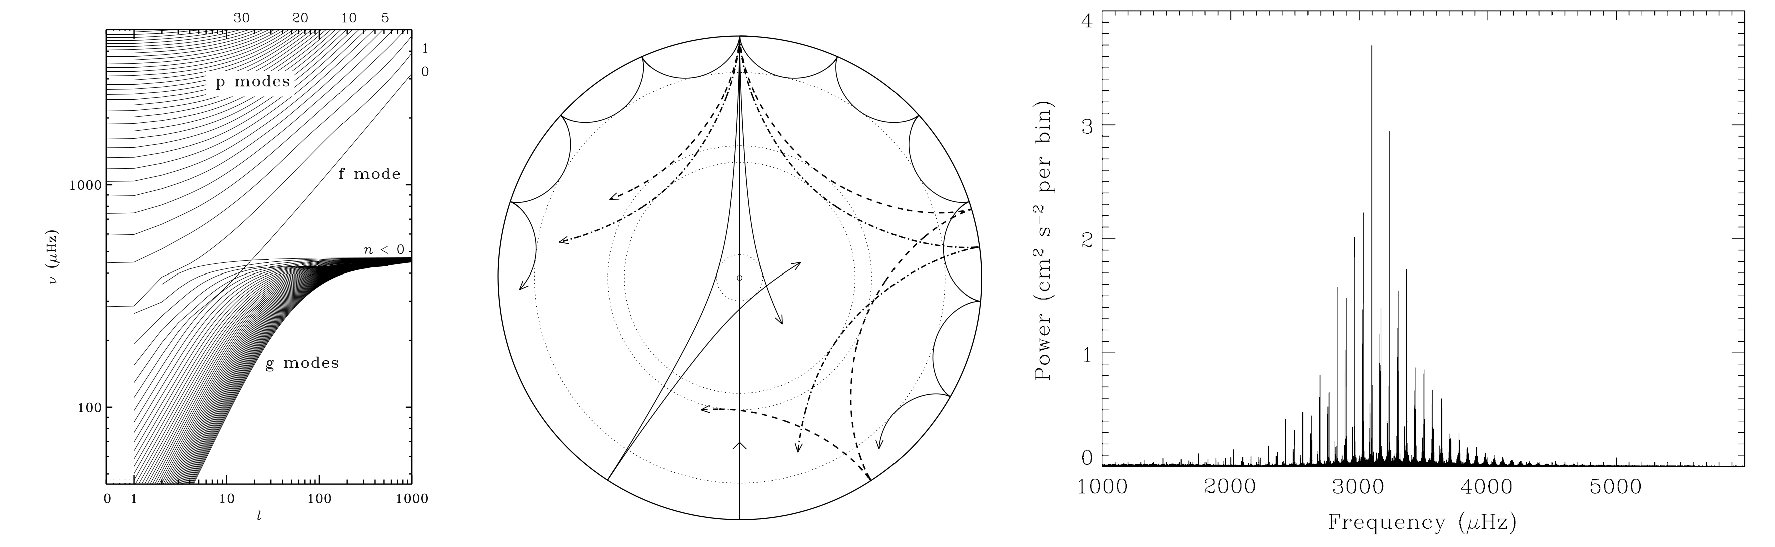
\includegraphics[width=\textwidth]{./figs/intro/asteroseismology.pdf}
\caption[Solar velocity power spectra.]
{
	Select images describing asteroseismology, taken from Ch.~1 of \citet{aerts&all2010}.
	(left, Fig.~1.6) Allowed frequency modes in a standard solar model.
	The upper part of the diagram is filled with p modes; frequency increases with overtone $n$ and spherical harmonic degree $\ell$.
	The lower part of the diagram is filled with g modes, whose frequency decreases with overtone $n$.
	(middle, Fig.~1.7a) Propagation of rays of sound waves in a cross-section of a Sun-like star.
	Shown are rays (in increasing order of penetration depth) of spherical harmonic degree of $\ell = \{75, 25, 20, 2\}$.
	(right, Fig.~1.9) A power spectrum of radial velocity variations for 9.5 years of data of the Sun-seen-as-a-star.
	Distinct peaks corresponding to p-modes (as in the left panel) can be seen.
	\label{fig:asteroseismology} 
}
\end{figure}





\subsection{The Solar Convective Conundrum}
\label{sct:convective_conundrum}
The outer 30\% of the Sun is a highly stratified convective envelope, and recent observations reveal that we lack a fundamental understanding of dynamics in this region.
Various helioseismic observations \citep{hanasoge&all2012, greer&all2015} detect convective velocity magnitudes which vary by two orders of magnitude.
Furthermore, these observations, as well as measurements of solar surface velocities \citep{hathaway&all2015}, have an unexpected absence of velocity at large spatial scales.
In short, we do not observe large-scale ``giant cells'' driven by buoyant motions deep in the solar convection zone.
These measurements, and the absence of giant cells, consitute the Solar Convective Conundrum.

Two primary hypotheses currently aim to explain the absence of giant cells: ``entropy rain'' and a rotationally constrained solar convective interior.
The entropy rain hypothesis, first suggested by \cite{spruit1997}, posits many theories over-predict the importance of upflows and that \emph{downflows} are predominantly responsible for carrying the solar luminosity across the solar convection zone.
Recent theory and simulations, including some of my own work, suggest that small, intense downflows can indeed traverse the entire convection zone intact and may be more important than upflows in solar-like convection \citep{brandenburg2016, kapyla&all2017, andersLB2019}.
To date, this work neglects magnetism and rotation, and it is unclear how these complicating effects interact with these fast, powerful downflows.
Meanwhile, the rotationally constrained interior hypothesis suggests that Coriolis forces dominate the dynamics of deep solar convection, and that these forces mask giant cells.
Simulations by \cite{featherstone&hindman2016a, featherstone&hindman2016b} show that as convective flows become more rotationally constrained, dominant convective velocities are pushed to smaller length scales.
However, rotational effects on simulations can be hard to quantify; some simulations which nominally rotate at the solar rate show \emph{anti-solar} differential rotation \citep{gastine&all2014}, and other rotationally constrained simulations exhibit Jupiter-like bands \citep{brun&all2017}.
Regardless, current results and hypotheses suggest that the interplay between downflows and rotational effects must be better understood in stellar convection.

\begin{figure}[ht!]
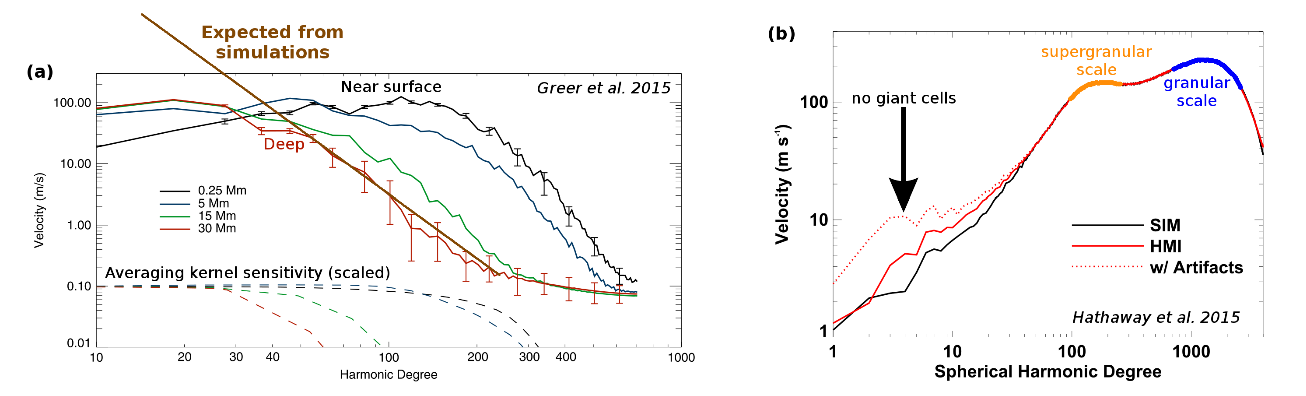
\includegraphics[width=\textwidth]{./figs/intro/conv_conundrum.pdf}
\caption[Solar velocity power spectra.]
{
	\citep[a, annoted Fig.~3 from][]{greer&all2015} Ring-diagram helioseismic observations of the solar velocity power spectrum at various depths.
	Here, velocity power decreases toward larger scales, unlike what is expected from simulations.
	\citep[b, annotated Fig.~8 from][]{hathaway&all2015} A spectrum of horizontal velocities at the solar surface, obtained using line-of-sight Doppler velocities.
	The length scales of surface granules and deeper supergranules appear as distinct features, but the hypothesized giant cells are not observed at low wavenumber.
	\label{fig:conv_conundrum} 
}
\end{figure}

\begin{figure}[ht!]
\includegraphics[width=\textwidth]{./figs/intro/solar_convection_scales.pdf}
\caption[Solar velocity power spectra.]
{
	(left) first-light image of the solar surface from DKIST (visible light [789 nm], covering 36.5 km$^2$).
	Bright, hot granules and relatively cool, dark intergranular lanes can be observed.
	Bright points occupying the center of intergranular lanes can also be seen \citep{vankooten&cranmer2017}.
	(right) Image of the solar surface from the Dutch Open Telescope (Ca II H line [396.8 nm]).
	The small-scale ``web'' of lights in this image trace out intergranular lanes.
	The large-scale web of lights roughly traces out the outlines of supergranules, the largest scale of convection that is observed at the solar surface.
	\label{fig:solar_convection_scales} 
}
\end{figure}

\begin{figure}[ht!]
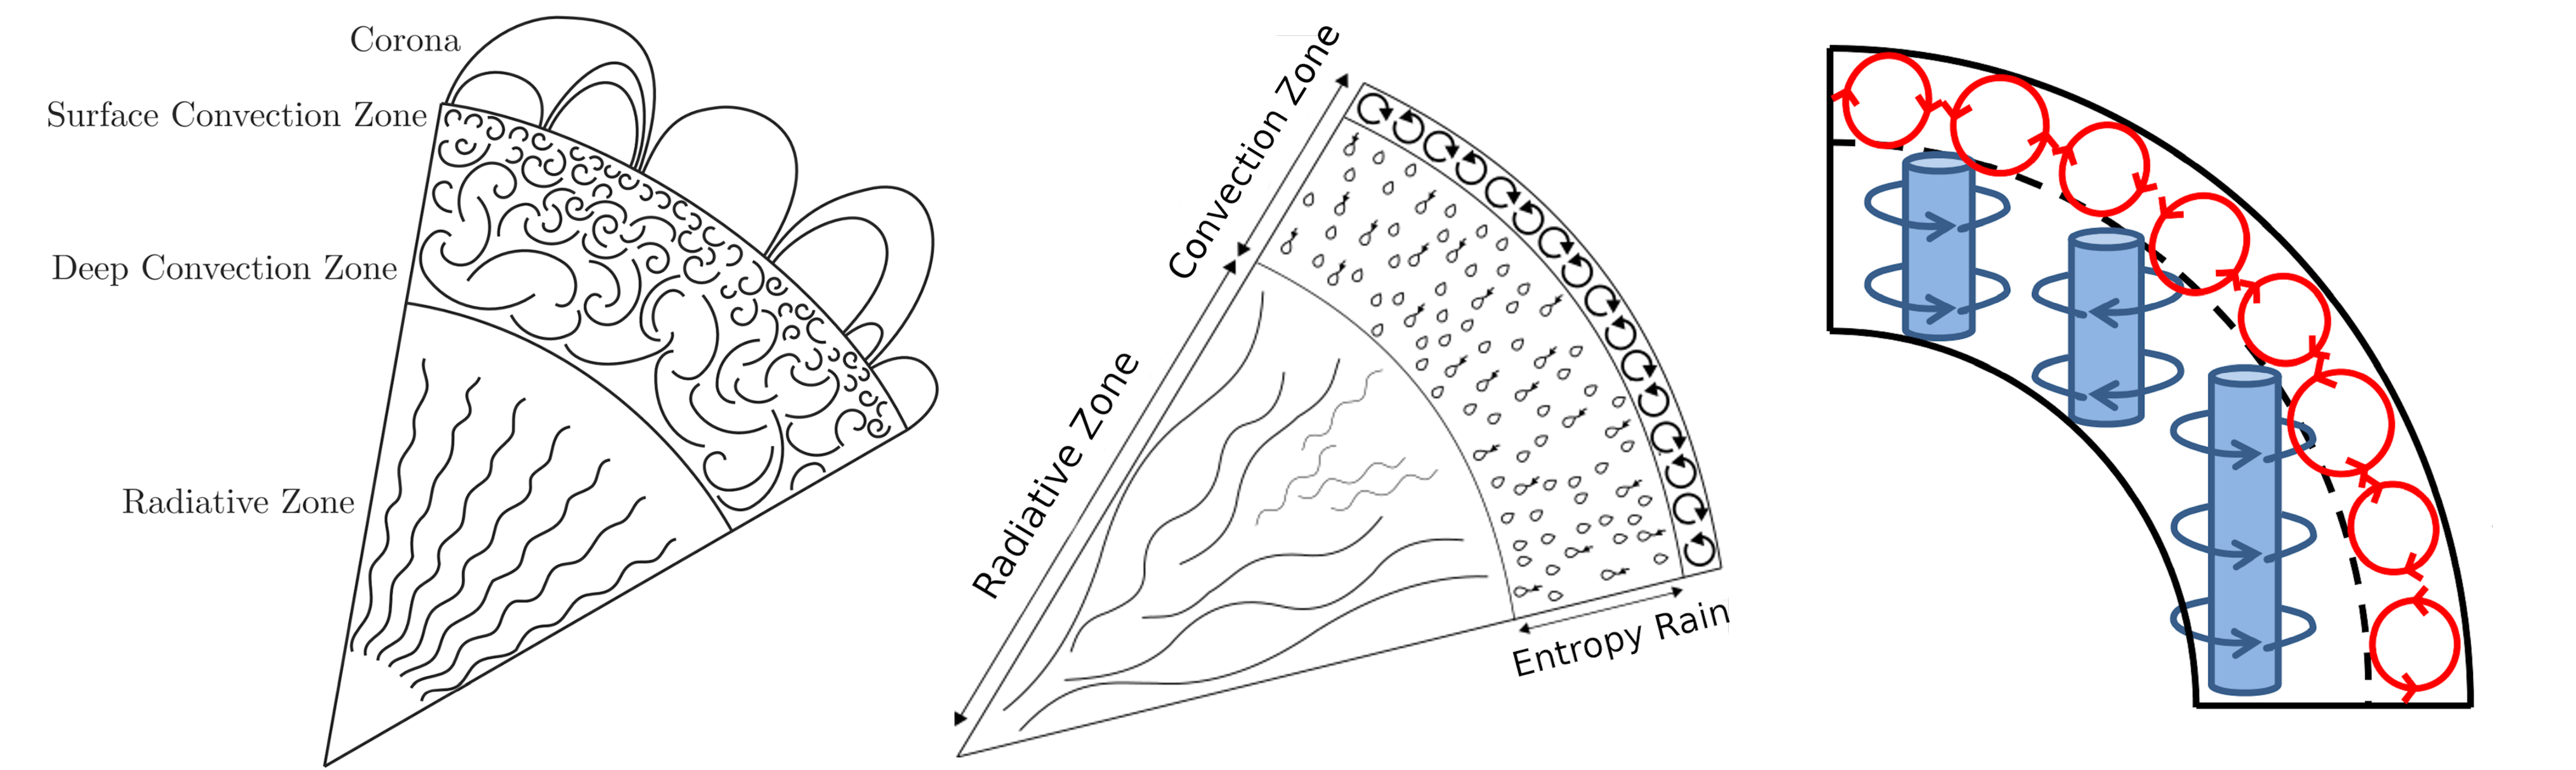
\includegraphics[width=\textwidth]{./figs/intro/conundrum_explanations.pdf}
\caption[Solar velocity power spectra.]
{
	(left, image courtesy of Daniel Lecoanet) The classic model of the solar interior.
	A deep radiative zone lies beneath a convective envelope; within the convective envelope, large convective cells are driven at the base, small cells are driven near the surface, and there is a gradient of cell sizes with increasing radius.
	(middle) The entropy rain picture of the solar interior.
	Beneath a thin surface convection zone, downflows or ``raindrops'' carry the solar luminosity from the solar surface to the base of the convection zone. 
	\citep[right, Fig.~3c of][]{featherstone&hindman2016b} The picture of the solar convection zone with a low-Rossby number, rotationally constrained interior.
	Rotational constraint increases with depth; below a certain depth, rotation dominates and convective cells give way to columns aligned with the global solar rotation.
	\label{fig:asteroseismology} 
}
\end{figure}




\section{A historical perspective on studies of convection}
Historically, experiments into the nature of convection have come from two distinct lines of motivation.
As is the case of the studies presented in this thesis, many studies into convection are motivated by the prevelance of convection in the natural world.
Convective experiments are also an ideal system in which to study driven turbulent flows.
These two motivations have led to a large variety of studies into the nature of convection, which I will attempt to briefly summarize here.
Generally, studies of \emph{turbulence} have focused on simple convective laboratory experiments or simulations in the Boussinesq regime, whereas astrophysically or geophysically motivated span from the same simple experimental setups to magnetohydrodynamic, global ``dynamo'' simulations in spherical domains.

\subsection{\RB convection}
The first controlled laboratory experiments of convection (or, a fluid layer heated from below and cooled from above) were performed by B\'{e}nard in 1900.
Over a decade later, the first \emph{theoretical} description of that convective layer was performed by Lord Rayleigh in 1916, at who first derived the Rayleigh number,
\begin{equation}
\text{Ra} = \frac{\alpha g L^3 (\Delta T)}{\nu \chi},
\label{eqn:rayleigh_number}
\end{equation}
where $\alpha$ is the coefficient of thermal expansion (describing how temperature and density fluctuations are related), $g$ is the gravitational acceleration, $L$ is the depth of the fluid layer, and $\Delta T$ is the temperature difference across the fluid layer domain, and $\nu$ and $\kappa$ are respectively the viscous and thermal diffusivities.
Ra is roughly the ratio of buoyant convective driving to viscous dissipation, and the pioneering work of these scientists in the field are the reason that Boussinesq thermal convection is widely known as \RB convection (RBC).
Together with geometric factors (the size and shape of the experimental domain), boundary conditions, and the Prandtl number (Pr = $\nu/\chi$), the Rayleigh number fully describes a convective system.
Ra is an ideal control parameter for a convective system, because it is a straightforward knob for convective driving: above some ``critical value,'' $\text{Ra} > \text{Ra}_{\text{crit}}$, a fluid layer should convect, and the more ``supercritical'' ($S = \text{Ra}/\text{Ra}_{\text{crit}}$) a layer is, the more turbulent the convection should be.
Furthermore, the value of $\text{Ra}_{\text{crit}}$ is independent of $\text{Pr}$ and is therefore independent of the specific fluid used in a convective experiment (e.g., in air Pr = 0.7 and in water Pr = 7).

Historical reviews of the development of studies of RBC can be found throughout the decades in e.g., \citet{busse1978, siggia1994, ahlers&all2009}.
In the simplest of terms, much of the research into RBC focuses on the behavior of heat transfer across a convective domain, quantified by the nondimensional Nusselt number (Nu),
\begin{equation}
\text{Nu} = \frac{\text{Evolved Convective Flux}}{\text{Comparison Hydrostatic Flux}} = \frac{\angles{w T - \chi \partial_z T}}{|\chi \Delta T / L|},
\end{equation}
where $w$ is the vertical velocity, and $T$ is the temperature field, and $\angles{}$ are a volume average over the convective domain.
The key historical question that has been asked is: how does Nu (and also the Reynolds number, Re) scale as Ra and Pr are changed?
The earliest theoretical description developed by \citet{malkus1954} asserts that the boundary layers of convective domains are always in a marginally stable state, and thus when the Rayleigh number is defined with $L = \delta$, the boundary layer thickness, it should always have a value of Ra$_{\text{crit}}$.
Such arguments lead to a classical scaling law of $\text{Nu} \propto \text{Ra}^{1/3}$, and similar scalings have been seen in experiments for decades.
More recently, in \citet{grossman&lohse2000} and following papers, a unifying theory of scaling behavior has been developed that is based around the dissipation of kinetic and thermal energy.
Each of these energy dissipations is split into a bulk and boundary layer component, due to the different force balances at work in the bulk or the boundary layers.
Scaling laws are then determined by where in the domain each type of energy is primarily dissipated, and this results in four regimes in parameter space (e.g., where kinetic energy is dissipated in the boundaries but thermal is dissipated in the bulk, and other permutations).
This theory, and a comparison to experimental and numerical results, are described in detail by \citet{ahlers&all2009}.
Regardless, a great number of studies have historically sought out the so-called ``ultimate regime'' of convection, which is the regime in which boundary layer dissipation is unimportant compared to the bulk, and some authors have recently claimed to have achieved such scalings \citep[see e.g.,][]{zhu&all2018}.

\subsection{Convective experiments that are closer to nature}
While modern and historical studies of RBC have allowed the community of convective modelers to understand convective experiments to a much greater degree, they do not contain all of the ``ingredients'' which are important to astrophysical or geophysical convection.
Numerous studies exist which aim to understand these additional complexities, ranging from studies which essentially study RBC with one extra component to studies with realistic radiiative transfer, magnetism, etc.

On the simpler end of this spectrum, the effects of rotation, and to a lesser extent magnetism, have been studied in the RBC context to great detail.
\citet{plumley&julien2019} provide an excellent overview of these fields.
In general, the presence of global rotation or a strong background magnetic field suppress convection, and thus increase the value of Ra$_{\text{crit}}$.
At low supercriticalities above Ra$_{\text{crit}}$, rotational (e.g., Coriolis) or magnetic forces dominant the convective flow balances.
As $S$ is increased, these forces become less important until eventually convective scaling laws return to their nonrotating or nonmagnetic forms.
Theoretical descriptions of these models often focus on understanding scaling laws in the rotationally- \citep[e.g.,][]{julien&all2012} or magnetically- \citep[e.g.,][]{cioni&all2000} dominated regime.
In this thesis (Ch.~\ref{ch:ro_p19}), we focus on the effects of rotationally-influenced convection in stratified atmospheres.

Outside of the realm of RBC, the field of convective research is less systematic and focused.
Atmospheric density stratification is one key ingredient of convection in geophysical and astrophysical applications.
The simplest stratified convection studies utilize a polytropic stratification, which has a linear temperatur profile and is therefore at least somewhat comparable to RBC.
The first study which determined how to find Ra$_{\text{crit}}$ in a polytropic atmosphere was \citet{unnoetall1960}, but the first dynamical simulations of polytropic convections could not be performed until those of \citet{graham1975}.
These early works focused on similar questions to those studied in the RBC community (how does Nu behave as Ra increases?) but were limited to a very small range of supercriticalities.
Subsequent studies into polytropic convection \citep[e.g.,][]{hurlburt&all1984, cattaneo&all1991} often focused more on the morphology of overall convective flows and the emergent nonlinear phenomena.
This trend continued as complicating physics were added in addition to stratification (e.g., rotation in \citet{brummell&all1996, brummell&all1998}, stably stratified layers in \citet{hurlburt&all1986, singh&all1995, brummell&all2002}, or magnetism/dynamo action in \citep{nordlund&all1992, brandenburg&all1996, tobias&all1998}).

As computational resources have continued to increase, so too have the complexity of convective simulations.
Modern ``dynamo simulations'' examine the evolution of rotating magnetohydrodynamic convection in spherical domains and have produced fascinating phenomenon.
These dynamo simulations regularly produce self-consistent differential rotation \citep{strugarek&all2018}, ``wreaths'' of magnetism \citep{brown&all2010}, magnetic cycles \citep{brown&all2011}, and more phenomenon.
These emergent phenomena parallel observed phenomena on the Sun and suggest that our fundamental understanding of the Sun's dynamo (that it is driven by turbulent motions in the convective zone) are correct.
However, these simulations are difficult to run and are so complex in and of themselves that they are essentially like observations in that it is easy to see what they produce, but hard to understand and predict how those phenomena occurred.

Dynamo simulations are not the only class of simulations which face this problem.
Small scale ``local'' simulations with realistic radiative transfer strikingly visually resemble solar surface convection and sunspots \citep{stein&nordlund1998, rempel&all2009, stein&nordlund2012, rempel2014}.
These simulations are visually resemble solar surface convection so convincingly that the raw data of e.g., \cite{rempel2014}'s simulations are being used directly as high-resolution observations of solar convection \cite[see e.g.,][and others]{vankooten&cranmer2017, shchukina&trujillo2019}.
While we study the flows in these simulations in great detail, they ultimately mostly just tell us the same thing that observations do: the solar surface convects, the photosphere is where the solar atmosphere becomes optically thin, and sunspots are regions of large magnetic field in the presence of this convection.

The ultimate goal of convective models in the context of solar or stellar convection is to understand how the solar dynamo operates so that we can eventually, hopefully, \emph{predict} its behavior.
The great numerical resources available to modern numericists have proven that we can simulate impressive things.
It is now crucial to simplify our simulations to conduct \emph{experiments} in which we study how specific pieces of convection behave \citep[such as in the studies of tachocline interactions of][]{wood&brummell2018}.
Through the knowledge gained in more focused studies, we can better predict the results of global simulations, and better build up a model of dynamo action, or other complex behavior in geo- or astrophysical convection.


\subsection{Mixing Length Theory \& Stellar Structure Models}
While the first analytical description of convection was performed by \citet{rayleigh1916}, the earliest formulation of a simple mixing length theory was derived by \citet{prandtl1925}.
The predecessor to most formulations of stellar mixing length thoery (MLT) used today are those of \citet{vitense1953} and \citet{bohm-vitense1958}.
Modern MLT has many branches, but the one described in Chapter 14 of \citet{weiss&all2004} and earlier versions of Cox \& Giuli's book provide an excellent and fundamental description of MLT.

MLT serves as a one-dimensional description of complex three-dimensional convective motions.
MLT assumes that, at a given stellar radius, the complex distribution of convective elements present can be modeled as an average convective element whose properties depend on the star's local structure.
Each of these elements is assumed to travel the ``mixing length,'' before depositing its thermodynamic signature into the surrounding matter and losing its identity.
As a result, hot elements transport warm material upward some mixing length, cold elements transport cold material downward some mixing length, and on average heat is transported outward, and a one-dimensional convective flux can be constructed.
While MLT is obviously an over-simplification of convective processes, it works qualitatively, and until recently it shows few noticeable disagreements with the observations available.
Furthermore, there is no widely accepted alternative description of convection to MLT, and so it is commonly used in the field as the only widely-accepted parameterization of convection.

State-of-the-art stellar strucuture models are produced by 1D codes like MESA \citep{paxton&all2011}, which depend on convective parameterizations like MLT.
Stellar structure models produced with MLT have aligned well with helioseismic observations for quite some time \citep{christensen-dalsgaard&all1996}, and disagreements between models and observations are generally less than a few percent \citep{serenelli&all2009}.
One particular area of weakness for these models has been problems due to ``near-surface effects'' \citep{kjeldsen&all2008}.
In short, MLT assumes that all convective flows are in perfect pressure equilibrium with their surroundings.
This assumption breaks down in the high-Mach number, highly superadiabatic surface layers of solar-like stars.
Recent efforts \citep{jorgensen&weiss2019, mosumgaard&all2020} have successfully coupled 1D stellar evolution models with thin, near-surface, 3D convective shells.
These studies have found that their realistic treatment of the highly adiabatic surface layers (via real 3D convective simulations) do indeed reduce errors in asteroseismic frequencies between models and observations.
However, we are still far from an adequate solution to this problem: 3D simulations are expensive, and cannot feasibly be coupled with 1D stellar structure models throughout the entirety of a stellar lifetime.
Regardless, these recent results do indeed suggest that MLT fails describe stellar convection in at least one situation (surface layers), and lay bare the need for either improved models or more efficient means of coupling simulations of convection with 1D models.

One additional weakness of 1D stellar structure models is that they often neglect complicating effects like magnetism and rotation.
MESA has incorporated diffusion of angular momentum to enable at least some basic models of rotating stars \citep{paxton&all2013}.
Furthermore, recent theoretical and simulation work have sought to understand how well mixing length theory describes rotating convection \citep{BDLithwick2014, currie&all2020}, and have shown good agreement between modified rotational MLTs and the results of 3D convective simulations.
The Sun exhibits differential rotation characterized by latitudinal variations in angular velocity within the solar convection zone \citep{thompson&all1996, schou&all1998}, and latitudinal differential rotation has now been observed in other stars \citep{benomar&all2018}.
At this time, I am unaware of any work which has sought to understand how differential rotation, but many theorists \citep[e.g.,][]{brun&all2017} are grappling to understand how differential rotation profiles like the Sun's are formed.
In Chapter~\ref{ch:ro_p19}, I will explore one fundamental study in rotating convection.

The effects of stellar magnetism on convection are less well-understood than rotation.
Recent theoretical work suggests that the topology of a star's magnetic field can induce variations in pulsational frequencies \citep{santos&all2018}, suggesting that magnetism should not be neglected.
A deep exploration of dynamo action or magnetoconvection in the stellar context is beyond the scope of this thesis, and I refer the reader to the reviews of \citet{brandenburg&subramian2005, charbonneau2010, charbonneau2014, brun&browning2017}.


\subsection{The Impossibility of Astrophysical Parameter Space}
\label{sct:nondimensional_parameters}
The Rayleigh number (Ra) is the most important nondimensional parameter used in describing experiments of convection.
Ra is roughly a measure of the ratio of the strength of buoyant convective driving to viscous dissipation.
In \RB convection, Ra is defined as in Eqn.~\ref{eqn:rayleigh_number}.
However, in such a form it is impossible to apply to astrophysical convection.
In acknowledging that the Boussinesq freefall velocity is $u_{\text{ff}} = \sqrt{\alpha g L \Delta T}$, one can see that the Rayleigh number is simply a product of the freefall Reynolds and P\'{e}clet numbers,
\begin{equation}
\Peff = \frac{u_{\text{ff}} L_z}{\chi}, \qquad
\Reff = \frac{u_{\text{ff}} L_z}{\nu},  \qquad
\text{Ra} = \Peff\Reff = \frac{u_{\text{ff}}^2 L_z^2}{\nu\chi}.
\end{equation}
Under this formulation, given an estimate of the diffusviites and MLT convective velocities, one can calculate an approximate value of Ra.
Also, in this formulation it is clear to see that Ra is in some ways a direct measure of how turbulent the convective motions are.

A perhaps more simple estimate for calculating Ra is to use a ``flux Rayleigh number,'' ($\text{Ra}_F$), which many authors use \citep[e.g.,][use an entropy-based formulation of one]{featherstone&hindman2016a}.
Ra$_F$ can be defined,
\begin{equation}
\text{Ra}_F = \frac{g L^4 F}{\rho T c_P \nu \chi^2},
\end{equation}
where $g$ is the gravity, $L$ is the length scale, $F$ is the flux, $\rho$ is the density, $T$ is the temperature, $c_P$ is the specific heat at constant pressure, $\nu$ is the kinematic viscosity, and $\chi$ is the thermal diffusivity.
This formulation can be derived from Eqn.~\ref{eqn:rayleigh_number} simply in a few steps.
First, assume that the temperature scale is defined based on the temperature gradient $\Delta T = L \grad T$.
Second, Assume that the flux in a corresponding static atmophere is carried entirely by radiative conductivity, $F = -\kappa \grad T$, where the conductivity relates to the diffusivity by $\kappa = \rho c_P \chi$.
Third, assume that the fluid is an ideal gas (pressure, $P = R\rho T$ for a constant $R$), and thus the coefficient of thermal expansion is $\alpha = -\partial_T \ln\rho  = T^{-1}$.
Under these assumptions, and multiplying the numerator and denominator of Eqn.~\ref{eqn:rayleigh_number} by $\kappa$, the definition of Ra$_F$ can be retrieved.

In order to understand the magnitude of Ra$_F$, I will now estimate its value for the mid solar convection zone.
The length scale of the solar convection zone is about $L = 200$ Mm, or about 30\% of the Sun's 700 Mm radius.
At the mid-CZ ($r \approx 600$ Mm), most (or at least about half) of the solar luminosity ($L_\odot \approx 3.85 \times 10^{33}$ erg/s) is carried by the convection.
Thus, $F = L_{\odot} / (4\pi r^2) \approx 8.5 \times 10^{10}$ erg/s/cm$^2$.
From a simple solar MESA model (a 1 $M_\odot$ star evolved to 4.5 Gyr), at the mid-CZ, 99.5\% of $M_\odot$ is located further radially inward, $T \approx 10^6$ K, $\rho \approx 0.05$ g/cm$^3$, $g \approx 3.78 \times 10^4$ m/s$^2$, and $c_P \approx 3.43 \times 10^{7}$ erg/K.

The diffusivities are a bit harder.
While this is not a perfect approximation, we can model the solar convection zone as a fully-ionized, 100\% Hydrogen fluid.
In this case, the Spitzer viscosity for a fully ionized gas applies \citep[Eqn.~5-54 of][]{spitzer1962},
\begin{equation}
\nu = (2.21 \times 10^{-15}) \frac{T^{5/2}}{\rho \ln \Lambda} \text{cm}^2/\text{s},
\end{equation}
for $T$ and $\rho$ in cgs units.
Here, $\ln\Lambda$ is the Coulomb logarithm, defined on page 34 of the 2019 edition of the plasma formulary for a fully ionized hydrogen gas as
\begin{equation}
\ln \Lambda = 23 - \ln\left(\frac{\sqrt{2\rho}}{\sqrt{m_P}T^{3/2}}\right),
\end{equation}
where $m_P$ is the mass of a proton in grams.
Under the diffusion approximation \citep[e.g., ch.~14.A-6 of][]{weiss&all2004}, the thermal conductivity is 
\begin{equation}
\kappa = \frac{16 \sigma_{\text{SB}} T^3}{3\rho k},
\end{equation}
where $k$ is the opacity and $\sigma_{\text{SB}} = 5.67 \times 10^{-5}$ erg/(cm$^2$ K$^4$ s).
A chi-by-eye estimate of the opacity in this region of the Sun \citep[from OPAL opacities and Fig.~3 of][]{paxton&all2011} is $k \sim 10^3$ cm$^2$/g.
Rearranging, we can solve for
$$
\chi = \frac{16 \sigma_{\text{SB}} T^3}{3\rho^2 c_P k}.
$$
Plugging in the temperature, density, opacity, etc.~of the mid-convection zone, we get roughly
\begin{equation}
\nu \approx 2.5 \,\text{cm}^2/\text{s}, \qquad
\chi \approx 3.5 \times 10^{6}\,\text{cm}^2/\text{s}.
\end{equation}
Note also that this means that the Prandtl number, Pr = $\nu/\chi \approx  10^{-6}$, and is generally very small in stellar interiors.
With these estimates of the diffusivity, we calculate an approximate solar Ra,
\begin{equation}
\text{Ra}_F\bigg|_{r=0.85 R_\odot} = \frac{g L^4 F}{\rho T c_P \nu \chi^2} \approx 10^{31}.
\end{equation}
Which is frankly enormous.

The largest values of Ra currently accessible to experiments is Ra$\,\approx 10^{15}$ \citep{zhu&all2018}, and those experiments are 2D, unstratified, Boussinesq, and possibly not properly numerically resolved.
The regime of very-high-Ra stellar convection is inaccessible using modern computational and laboratory tools.
However, it is still possible to study convection as a function of Ra to learn how convection behaves as we exit the laminar regime and step towards the high-Ra, astrophysically interesting regime.


\section{Numerical Methods}
\label{sct:numerics}


\subsection{Direct Numerical Simulations vs.~Large Eddy Simulations}
Direct Numerical Simulations (DNS) are simulations in which the Navier-Stokes equations are evolved in their entirety without any model for the turbulence, and the term was first coined by \citet{orzag1970}.
Due to the fact that they resolve all spatial scales down to the turbulent viscous cutoff scale, DNS were until recently limited to studies of relatively laminar flows.
As computational resources have expanded over the past decades, so too have the regions of turbulent parameter space available for probing through DNS.


Large Eddy Simulations (LES) were first proposed by \cite{smagorinsky1963}, and first explored numerically by \citet{deardorff1970}.
An excellent argument in favor of the use of LES is laid forth by \citet{miesch&all2015}, and I refer the reader there for a more thorough exploration of this topic than will be undertaken here.
In short, the central premise of LES is that large scale motions dominate both the turbulent transport and energy budget of a fluid system such as the solar convection zone, so a numerical simulation that captures those scales should realistically describe the real system.
However, this premise hinges on the fact that the unresolved small scales are realistically taken into account, and these small scale motions are generally either included explicitly as subgrid-scale (SGS) models or handled implicitly through numerical dissipation.
A given simulation can capture length scales which vary between $L$, the large-scale size of the simulation domain, and $\ell$, a small-scale set by e.g., the grid resolution.
If $\ell \leq \ell_{\text{diss}}$, the dissipation length scale, then the simulation is a DNS -- it explicitly captures scales down to (and possibly below) the dissipation scales.
In an LES, the goal is to set $L$ to the largest scales present in the system of interest, and to set $\ell_{\text{diss}} \ll \ell \ll \ell_{\text{max}}$, where $\ell_{\text{max}}$ is the dominant length scale of e.g., convective velocities being modeled in the system.
By doing so, in theory a realistic description of the sytem is attained while using many fewer computational resources than would be required to resolve the largest scales in a DNS (which also must achieve small enough grid scales to resolve $\ell_{\text{diss}}$).

DNS and LES are two different tools to be used for different problems.
In the physics community where \RB convection is studied, DNS are the tool of choice.
There, simulations are often compared either directly or indirectly with experimental data.
A great deal of interest is taken in ensuring that the boundary layers are resolved \citep{shishkina&all2010} due to the dominance of boundary layers in suppressing heat transport throughout the parameter space available to DNS and experiments \citep{ahlers&all2009}.
When applied to astrophysics, DNS generally aim to understand how flow properties behave as turbulence is increased.
These scaling laws can then be extrapolated out to astrophysical quantities (which are often many decades away from the most turbulent values achievable in DNS).
In short, in studies of astrophysics, it is acknowledged that DNS cannot achieve a model of the true astrophysical system of interest, but can instead provide insight into the behavior of similar systems at less extreme parameters.
The goal of LES is to study dynamics in a system which is as close to a realistic model of the astrophysical system of interest as can be achieved.
However, LES are senitive to choices of how to model SGS effects.
Some recent studies suggest that these two approaches should not be seen as an ``either or'' choice but a ``both and'' \citep{mellado&all2018}.
In other words, DNS studies can be used to accurately model small scales, and those results can better inform SGS choices of LES.

Regardless, both DNS and LES have benefits and limitations, and it is important that the simulator be aware of the limitations of their tool of choice.
All of the simulations conducted in this work are DNS.

\subsection{Finite Element vs. Spectral Methods}
The simplest and most straightforward way of modeling a physical system numerically is through the use of finite element, finite volume, and finite difference methods.
In these systems, physical space is discretized into a series of coordinates, and the values of relevant quantiies (velocity, density, etc.) are tracked at each of those locations, and derivatives are computed based on the values of quantities in neighboring grids.
Finite volume codes can be used to model problems in complex geometries, but can be difficult to implement for complex equations and converge slowly as the simulation resolution is increased \citep{burns&all2019}.
Some modern examples of finite volume codes used in astrophysical fluid modeling are the Stagger\footnote{\url{https://starformation.hpc.ku.dk/?q=node/18}} \citep{galsgaard2011}, PLUTO\footnote{\url{http://plutocode.ph.unito.it/}} \citep{mignone&all2012}, Athena/Athena++\footnote{\url{https://princetonuniversity.github.io/athena/}} \citep{stone&all2008, stone&all2019}, the Pencil Code\footnote{\url{http://pencil-code.nordita.org/}} \citep{brandenburg&dobler2010}, and MUSIC\footnote{\url{https://empslocal.ex.ac.uk/tofu/}} \citep{goffrey&all2017}.

Spectral methods, on the other hand, discretize important quantities by expanding them over a set of bases functions.
Common basis choices include Fourier series and Chebyshev polynomials.
Such methods can highly accurately follow the value of evolving fields at all spatial locations within a domain, but are generally restricted to simple geometries (Cartesian, cylindrical, and spherical domains).
The code used to perform all simulations in this thesis, Dedalus\footnote{\url{http://dedalus-project.org/}} (described below in sct.~\ref{sct:dedalus}), is a \emph{pseudo}spectral code.
This means that, while solving equations, all linear equation terms are handled in a fully spectral sense.
Nonlinear terms are dealiased, projected onto a finite volume domain, and analyzed. 
Pseudospectral methods can be much more efficient than spectral methods in the analysis of certain terms.
Some other modern codes which employ spectral methods are Rayleigh\footnote{\url{https://geodynamics.org/cig/software/rayleigh/}}, MagIC\footnote{\url{https://magic-sph.github.io/}} \citep{wicht&all2017}, SNOOPY\footnote{\url{http://geoffroy-lesur.org/snoopy.html}} \citep{lesur2015}, and ASH (closed source).

A benchmark comparing Dedalus' pseudospectral methods to Athena's finite volume methods for a turbulent, nonlinear Kelvin-Helmholtz instability is explored by \citet{Lecoanet_et_al_2016_KH}.


\subsection{Timestepping: Implicit \& Explicit methods}
\label{sct:intro_timestepping}
The most common class of timestepping methods used are explicit timestepping methods.
In these methods, the future state of the system is solved for as a function of the current state of the system and some timestep size, $\Delta t$.
While these methods are the simplest to implement, they are inefficient at solving stiff problems in which there are two different flows which act on very different timescales.
Specifically, in order to ensure that timestepping errors remain small, it is important that timesteps which are ``too large'' are not taken.
Mathematically, the size of the largest possible timestep which can be taken is specified by the Courant-Friedrichs-Lewy (CFL) condition,
\begin{equation}
C = \frac{u \Delta t}{\Delta x} \leq C_{\text{max}},
\end{equation}
where $C$ is the Courant number, $C_{\text{max}}$ is typically O(1) for explicit methods, $\bm{u}$ is the fluid velocity magnitude, and $\Delta X$ is the grid spacing of a simulation \citep{cfl1967}.

Implicit timestepping methods, on the other hand, solve a linear algebraic system that involves both the current and the future timestep.
These methods are as a general rule more memory intensive than explicit methods and are also more difficult to implement.
The MUSIC code is one of the first astrophysical codes to offer the capability of studying stellar convection which utilize a fully implicit timestepper.
Since implicit methods are not bound as strongly by the CFL condition, there has been great optimism that the implementation of implicit methods could allow numericists to simulate convection over many dynamical timescales using a modest number of timesteps.
Unfortunately, as discovered by \citet{viallet&all2011, viallet&all2013, viallet&all2016}, implicit methods do not achieve an accurate solution if the superstep the CFL of all simulation flows.
Specifically, it was found that implicit methods must take short enough timesteps in order to resolve nonlinear advective flows.

Mixed implicit-explicit (IMEX) methods have been growing in popularity in recent years.
These methods utilize the best parts of both implicit and explicit methods.
Generally, these methods handle linear terms implicitly, thereby superstepping CFL conditions on linear waves or other linear system solutions.
These methods then handle their nonlinear terms explicitly, using significantly less memory than nonlinear implicit methods.
All of the simulations presented in this thesis utilze IMEX methods.


\subsection{Equation Formulation: From Complexity to Simplicity}
\label{sct:intro_equations}
The equations which are the cornerstone of any fluid dynamical study are at some point an approximation.
Even the fully compressible Navier-Stokes equations,
\begin{gather}
\frac{\partial \rho}{\partial t} + \Div{\rho\bm{u}} = 0 
\label{eqn:intro_fc_continuity}
\\
\frac{\partial \bm{u}}{\partial t} + \bm{u}\cdot\grad\bm{u} = -\frac{1}{\rho}\grad P + \bm{g} + \frac{1}{\rho}\Div{\stressT},
\label{eqn:intro_fc_momentum}
\end{gather}
are an approximation upon kinetic theory for how an ensemble of particles behaves.
Here, $\rho$ is the fluid density, $\bm{u}$ is the bulk fluid velocity, $P$ is the pressure, $\bm{g}$ the gravity, and $\stressT$ the viscous stress tensor.
It is likely crucial that a simulation studying the near-surface layers of the Sun---where the Mach number is high and compressibility effects are important---use a fully compressible equation set, as formulated above.
However, in certain limits, it is often useful to approximate these equations even further.

\subsubsection{The Lantz-Braginsky-Roberts (LBR) Anelastic Equations}
One of the most commonly used approximations of the fully compressible equations in astrophysics is the Anelastic approximation.
Under this approximation, density fluctuations are assumed to be small such that Eqn.~\ref{eqn:intro_fc_continuity} becomes
\begin{equation}
\Div{\rho_0 \bm{u}} = 0,
\label{eqn:intro_an_continuity}
\end{equation}
where here $\rho_0$ is the background atmospheric stratification.
This approximation essentially says that density fluctuations away from $\rho_0$ are so small that they can be neglected.
While many formulations of the Anelastic equations have been used, perhaps one of the ``best'' is the Lantz-Braginsky-Roberts (LBR) formulation attributed to \citet{lantz1992} and \citet{braginsky&roberts1995}.
This formulation both conserves energy \citep{brown&all2012} and can be derived from Lagrangian constraints \citep{vasil&all2013}.
In this formulation, the momentum equation (Eqn.~\ref{eqn:intro_fc_momentum}) becomes
\begin{equation}
\frac{\partial \bm{u}}{\partial t} + \bm{u}\cdot\grad\bm{u} = -\grad \varpi - \frac{S_1}{c_P} \bm{g} + \frac{1}{\rho_0}\Div{\stressT},
\label{eqn:intro_an_momentum}
\end{equation}
where $\varpi \equiv P_1 / \rho_0$ is the reduced pressure (here $P_1$ are pressure fluctuations away from the background pressure profile $P_0$, which is assumed to be in hydrostatic equilibrium) and the specific entropy is given by the linearized ideal gas equation of state,
$$
\frac{S_1}{c_P} = \frac{1-\gamma}{\gamma}\frac{P_1}{P_0} + \frac{T_1}{T_0},
$$
where $T$ is the temperature.

One benefit of anelastic approximations such as the one here is that they are \emph{soundproof}.
In other words, these equations are not stiff: acoustic waves are explicitly filtered out of the linear solution of these equations, so simulations of low Mach number flows can be performed using explicit timestepping techniques without having to take prohibatively small timesteps that follow the sound waves.
Anelastic equation formulations have historically been used in many global simulation models (ASH and Rayleigh both use an anelastic equation formulation).
More recently, implicit-explicit (IMEX) timestepping methods have enabled low Mach number simulations under the \emph{fully compressible} equations which are not bound by the CFL.
If these methods become more prevalent, it is possible that Anelastic approximations may become a thing of the past.
Regardless, some comparisons of fully compressible low Mach number dynamics and Anelastic dynamics have shown remarkable agreement between the two equation sets \citep[see e.g.,][and chapter \ref{ch:alb19}]{lecoanet&all2014, andersLB2019}.
As such, due to their simplicity, anelastic models will likely continue to find use in theoretical descriptions of low Mach number flows.

\subsubsection{The Boussinesq approximation}
The simplest possible approximation in which buoyantly driven flows are frequently studied is the Boussinesq approximation.
The limits of this approximation were famously explored by \citet{spiegel&veronis1960}.
The Boussinesq approximation applies when thermodynamic and density fluctuations are small compared to the background (as in the Anelastic approximation), \emph{and} when the vertical dimension of the fluid being studied is significantly smaller than the atmospheric scale height.
In other words, the Boussinesq approximation applies when the fluid is nearly incompressible, but where buoyant forces are still important.
Under these conditions, the continuity equation (Eqn.~\ref{eqn:intro_fc_continuity}) becomes the incompressibility constraint,
\begin{equation}
\DivU = 0,
\label{eqn:intro_incompressibility}
\end{equation}
and the density is assumed to be a constant ($\rho_0$) everywhere except on the gravitational term in the momentum equation, where it is $\rho = \rho_0 + \rho_1$.
Assuming that the background atmospheric profile is in hydrostatic equilibrium $-\grad P_0 + \rho_0 \bm{g} = 0$, and adopting the boussinesq approximation for density fluctuations on the gravitational term,
\begin{equation}
\rho_1 = \rho_0\alpha T_1,
\end{equation}
where $\alpha$ is the coefficient of thermal expansion and $T_1$ is temperature fluctuations away from background temperature profile.
The boussinesq momentum equation is
\begin{equation}
\frac{\partial \bm{u}}{\partial t} + \bm{u}\cdot\grad\bm{u} = -\grad \varpi - \alpha T_1 \bm{g} + \nu \grad^2 \bm{u},
\label{eqn:intro_bouss_momentum}
\end{equation}
where $\varpi$ is a reduced pressure as in the anelastic case, $\nu$ is the viscous diffusivity (in units of cm$^2$/s), and the viscous term simplifies into a Laplacian due to the incompressible constraint.

Mathematically, the similarity between Eqns.~\ref{eqn:intro_an_momentum} and \ref{eqn:intro_bouss_momentum} is striking.
Both have a straightforward buoyant term which makes warm perturbations rise and cool perturbations fall.
Both have a reduce pressure gradient which acts as a Lagrangian multiplier to enforce a constraint on the flow (Eqns.~\ref{eqn:intro_an_continuity} and \ref{eqn:intro_incompressibility}, see \citet{vasil&all2013} for a more thorough discussion).
The simplicity of these equations allows for more complete analytical manipulation of the equation, which in turn allows for the development of simple, testable hypothesis for application in DNS.

Throughout this thesis, all three of these levels of approximation will be used.
In Chs.~\ref{ch:ab17} and \ref{ch:ro_p19}, fully compressible convection will be studied.
In Ch.~\ref{ch:alb19}, the evolution of low Mach number fluid parcels will be analyzed using both fully compressible and anelastic simulations.
In Chs.~\ref{ch:abo18} and \ref{ch:FT20}, convection under the Boussinesq approximation will be examined.

\subsection{Dedalus: A pseudospectral toolkit}
\label{sct:dedalus}
Dedalus is an open source Python package which allows the user to apply pseudospectral and spectral methods to solve arbitrary partial differential equation sets.
These equation sets are generally solved in Cartesian domains, although select cylindrical domains are available, and an alpha version of Dedalus in spherical domains has been tested and is available \citep{vasil&all2019, lecoanet&all2019}
While the full functionality of Dedalus is covered in detail in its recently released methods paper \citep{burns&all2019}, I will briefly cover some of its functionality which enabled the work in this thesis.

\subsubsection{Arbitrary Equation Sets}
Dedalus users input sets of partial differential equations into Dedalus in a plain text format.
This means that using any of the the three equation sets covered in Section \ref{sct:intro_equations} is straightforward, and going from initial implementation of a new set of equations, to debugging those equations, to getting science results from those equations is a fast process.
As an illustrative example, take the boussinesq equations in two dimensions:
\begin{gather}
\DivU = 0, \\
\frac{\partial \bm{u}}{\partial t} + \bm{u}\cdot\grad \bm{u} = -\grad\varpi + \alpha g T_1 \hat{z} + \nu \grad^2\bm{u}, \\
\frac{\partial T_1}{\partial t} + \bm{u}\cdot\grad T_1 + w\frac{\partial T_0}{\partial z} = \chi \grad^2 T_1.
\end{gather}
While these equations \emph{*should*} generally be nondimensionalized before implementation in a computational system in order to better condition the numerical system, I will carry forward with these dimensional values.
In Dedalus, it is common to use a Chebyshev basis in the vertical direction, allowing for arbitrary boundary condition specification at the top and bottom of the domain.
The horizontal directions are usually taken to be periodic.
In the Chebyshev direction, it is crucial that the equations are entered in a first-order formalism.
For a two-dimensional problem with velocity $\bm{u} = u\hat{x} + w\hat{z}$, the full equation set is
\begin{align}
&u_z = \frac{\partial u}{\partial z}, \label{eqn:dedalus1} \\
&w_z = \frac{\partial w}{\partial z}, \\
&T_{1,z]} = \frac{\partial T_1}{\partial z}, \\
&\frac{\partial u}{\partial x} + w_z = 0, \\
&\frac{\partial u}{\partial t} + u\frac{\partial u}{\partial x} + w u_z = -\frac{\partial \varpi}{\partial x} + \nu \left(\frac{\partial^2 u}{\partial x^2} + \frac{\partial u_z}{\partial z}\right),\\
&\frac{\partial w}{\partial t} + u\frac{\partial w}{\partial x} + w w_z = -\frac{\partial \varpi}{\partial z} + \alpha g T_1 + \nu \left(\frac{\partial^2 w}{\partial x^2} + \frac{\partial w_z}{\partial z}\right),\\
&\frac{\partial T_1}{\partial t} + u\frac{\partial T_1}{\partial x} + w T_{1,z}  + w \frac{\partial T_0}{\partial z} = \chi \left(\frac{\partial^2 T_1}{\partial x^2} + \frac{\partial T_{1,z}}{\partial z}\right) \label{eqn:dedalus7}.
\end{align}
Given a Dedalus \texttt{problem} object, these equations can straightforwardly specified through text strings as follows:
\begingroup
	\fontsize{9.7pt}{9pt}\selectfont
	\begin{verbatim}
problem.add_equation("uz  - dz(u)  = 0")
problem.add_equation("wz  - dz(w)  = 0")
problem.add_equation("T1z - dz(T1) = 0")
problem.add_equation("dx(u) + wz   = 0")
problem.add_equation("dt(u) + dx(p)        - nu*(dx(dx(u))  + dz(uz))  = -u*dx(u)  - w*uz")
problem.add_equation("dt(w) + dz(p) + C*T1 - nu*(dx(dx(w))  + dz(wz))  = -u*dx(w)  - w*wz")
problem.add_equation("dt(T1) + w*T0z      - chi*(dx(dx(T1)) + dz(T1z)) = -u*dx(T1) - w*T1z")
	\end{verbatim}
\endgroup
In the above equations, terms are organized such that all linear terms are located on the lefthand side of the equations.
The righthand side of the equations is reserved for nonlinear terms.
In the above equations, the constant \texttt{C} is $\alpha g$ in the above equations.

It is clear to see that, from a user perspective, equation entry in Dedalus is straightforward.
However, the most powerful aspect of this simple equation entry is that is is trivial to add additional pieces of physics to these systems.
For example, if I wanted to expand this system to study doubly-diffusive convection, I would only have to modify the above equation set by adding a solute evolution equation and by changing the buoyancy term in the vertical momentum equation appropriately.
Such a modification could be performed in a number of minutes.
This extreme flexibility has in large part enabled the broad and somewhat disparate scientific applications explored in this thesis.

Throughout the rest of this section, I will use these equations as a representative example of the abilities of Dedalus.

\subsubsection{Three types of solvers}
One of the benefits of the Dedalus framework is that a block of code that solves a given set of equations, such as those specified in Eqns.~\ref{eqn:dedalus1}-\ref{eqn:dedalus7}, multiple types of solvers can be used.
Dedalus can solve Initial Value Problems, Eigenvalue problems, and Boundary Value Problems.
All of these solving capabilities were taken advantage of during this thesis, and I will briefly describe them below.

\paragraph{Initial Value Problems,} or IVPs, are the most common type of solver taken advantage of in this thesis.
When we solve an IVP in Dedalus, we are solving a DNS.
These problems take an equation set, and, given a set of initial conditions and boundary value problems, take steps forward in time.
It is up to the user to determine what an appropriate stop conditon is, and this is typically a quantity of time that it is desired that the simulation runs for.

\paragraph{Eigenvalue Problems,} or EVPs, have also been utilized in this thesis.
The Rayleigh number, or the ratio of buoyant driving to viscous dissipation, is the primary control parameter in our convective experiments.
We have primarily used EVPs to find the critical value of the Rayleigh number, Ra$_{\text{crit}}$, for our convective systems.
Dedalus performs an EVP on our above system of equations in the following steps:
\begin{enumerate}
\item It first ensures that the system is a linear system.
It does this by setting all variables (\texttt{u, uz, w, wz, T1, T1z,} and \texttt{p}) equal to zero and evaluating the RHS of each equation.
If all of the RHS values evaluate to zero under the assumption that all variables are zero, then the system is assumed to be linear.
\item The user assumes that each of the variables grows proportionally to $e^{i\omega t}$, and sets a substitution so that \texttt{dt(A)}$\rightarrow$\texttt{i$\omega$ A} for each variable \texttt{A}.
The user also generally wants to solve the EVP for a specific horizontal wavenumber, assumes that all fields can be expressed as a constant times $e^{i k_x x}$, and sets \texttt{dx(A)}$\rightarrow$\texttt{i$k_x$ A} for each variable \texttt{A}
\item Under these approximations, the above equation system can be expressed as the linear algebraic system,
\begin{equation}
\begin{bmatrix}
-\partial_z 		& 0 					& 0 					& 1 			& 0 			& 0 				& 0 \\
0    				& -\partial_z 			& 0 					& 0 			& 1 			& 0 				& 0 \\
0    				& 0 					& -\partial_z 			& 0 			& 0 			& 1 				& 0 \\
ik_x 				& 0 					& 0 					& 0 			& 1 			& 0 				& 0 \\
i\omega + \nu k_x^2 & 0						& 0						& \nu\partial_z & 0				& 0 				& i k_x \\
0					& i\omega + \nu k_x^2	& -\alpha g				& 0				& \nu\partial_z & 0 				& \partial_z \\
0					& \partial_z T_0		& i\omega + \chi k_x^2	& 0				& 0				& \chi\partial_z	& 0
\end{bmatrix}
\begin{bmatrix}
u \\ w \\ T_1 \\ u_z \\ w_z \\ T_{1,z} \\ p
\end{bmatrix}
= \bm{0},
\end{equation}
In this work, the eigenvalue we have always been interested in is $\omega$, describing with its imaginary component whether the solution experiences exponential growth (convection) or exponential decay (not convection).
In solving for this eigenvalue, Dedalus takes the determinant of the 7x7 matrix displayed above given a set of physical values (e.g., $k_x$, $\nu$, $\chi$), and sets that determinant equal to zero to solve for $\omega$.
\end{enumerate}

\paragraph{Boundary Value Problems,} or BVPs, have found some use in this thesis.
Usually we solve one-dimensional boundary value problems in the $z$ direction, and therefore use a simpler set of equations than the aforementioned equation set.
In Dedalus, BVPs are solved using a newton solver.
Given an initial guess for the answer as a function of height, Dedalus iteratively attempts to shoot the solution closer to one which satisfies both the equations and boundary conditions.






